\subsection{Analytical Model}\label{sec:network:performance_model:analytical_model}
This section introduces a performance model for quantifying power drain against signalling load.
The model allows researchers and application developers to evaluate analytical and empirical traffic distributions, deriving metrics for signalling and power drain in order to predict the impact of yet unimplemented applications or planned network configurations.

After presenting the system description, we derive the state distribution and the average frequency of state transitions for a Two State Model, e.g. for proprietary fast dormancy implementations of smart-phone vendors~\cite{NSN2011}. 
Afterwards, we extend the model to include \gls{RRC_FACH} for regular \gls{3G} networks.
Finally, we define simple metrics for signalling load and power drain.

\newcommand{\PacketIAT}{A\xspace}

\subsubsection*{Mobile \headershortacr{RAN} System Description}\label{sec:network:performance_model:analytical_model:system_description}
We consider a \gls{UE} which sends and receives a sequence of data packets via a \gls{3G} \gls{UMTS} network.
As discussed in \refsec{sec:network:background:umts_rrc}, the arrival process of the packet transmissions determines the \gls{RRC} states of the \gls{UE}.
However, the direction of packets, i.e. whether they originate from the \gls{UE} or the NodeB, has no impact on the \gls{RRC} states, as the states depend solely on traffic activity.
Due to the high impact of \gls{RRC} states on traffic patterns, we do not consider packet sizes in this model.
In real \gls{UMTS} networks very small packets might be treated differently for \gls{RRC} states, but we neglect this both for simplicity reasons and as the impact of packet sizes is highly network operator specific~\cite{Qian2010a}.
Furthermore, \gls{RRC} state transitions are complex procedures depending on implementation details of the \gls{UE}, the specific \gls{UMTS} release, and the configurations by the network operator.
In order to keep our model simple, but realistic, we reduce the set of standardised \gls{RRC} states and the state transition triggers in the following ways. 

In a first step we consider the Two State Model: \gls{RRC_idle} and \gls{RRC_DCH} as shown in \reffig{fig:network:background:rrc_state_machines:two_states}.
The \gls{UE} switches to \gls{RRC_DCH} to transmit or receive data and after an inactivity period of duration \TDCH, it switches back to \gls{RRC_idle}. 
The motivation for the two states \gls{RRC} scenario is twofold.
First, it serves for illustration purposes.
We derive the model step-by-step in this simple scenario to explain the ideas behind the equations.
Then, the ideas can be easily transferred to the more complex Three State Model.
Second, the scenario is of practical relevance since proprietary implementations of the fast dormancy concept can be modelled as the Two State Model, as discussed in \refsec{sec:network:background:umts_rrc}.
Furthermore, this model is very similar to the one found in \gls{LTE} systems.
In \gls{LTE}, only a distinction between connected and disconnected states can be found, which maps to the \gls{RRC_idle} and \gls{RRC_DCH} states discussed in this model.

In our model we aggregate both packets sent and received by the \gls{UE} in the packet arrival process, which is assumed to be a renewal process, i.e. a process  with identical and independently distributed inter-arrival times, described by the random variable \(\PacketIAT\) as shown in~\reffig{fig:network:performance_model:system_description:arrival_process}.
Thus, the probability that the time between two consecutive packets is at most \(t\) is \(P(\PacketIAT \leq t) = \PacketIAT(t)\).
This assumption is validated in \refsec{sec:network:performance_model:validations} using the application measurements obtained in \refsec{sec:network:network_traces:numerical_results}.

The packet arrivals determine the \gls{RRC} state of the \gls{UE} and the corresponding transitions. Therefore, the packet arrival process can be seen as a modulating process, c.f. \cite{TranGia1983,TranGia1988}, while the state and the signalling process represent modulated, i.e., resulting processes.

\begin{figure}
  \centering
  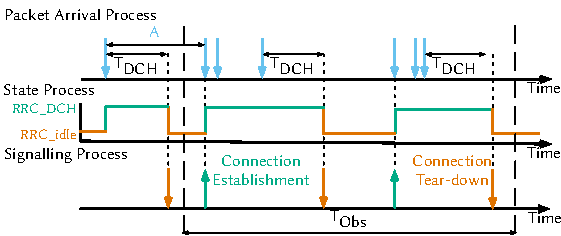
\includegraphics{network/performance_model/analytical_model/figures/arrival_process}
  \caption{Relation of packet arival process \(\PacketIAT\), state process, and signalling process in the Two State Model.}
  \label{fig:network:performance_model:system_description:arrival_process}
\end{figure}

\subsubsection*{Two State Model}\label{sec:network:performance_model:analytical_model:two_states}

\newcommand{\RRCState}{S\xspace}
\newcommand{\PacketIATDensity}{a\xspace}
\newcommand{\RRCStateRealization}{s\xspace}
\newcommand{\ObservationInterval}{T_{\text{Obs}}\xspace}
\newcommand{\ObservationPoint}{t^*\xspace}
\newcommand{\ObservationIntervalDensity}{q\xspace}
\newcommand{\ObservationIntervalLength}{\tau\xspace}
\newcommand{\NormalisationConstant}{c_0\xspace}
\newcommand{\NObservedPackets}{n_{\text{P}}\xspace}

\paragraph*{Connection State Distribution}
First, we are interested in the state distribution \(P(\RRCState=\RRCStateRealization)\), i.e., the fraction of time the \gls{UE} spends in state \(\RRCStateRealization\in\{\gls{RRC_idle},\gls{RRC_DCH}\}\) for a given inter-packet time \(\PacketIAT\).
For this purpose, we define an observation interval \(\ObservationInterval\), depicted in \reffig{fig:network:performance_model:system_description:arrival_process}, which is assumed to be larger in orders of magnitude than the average packet inter-arrival time \(E[\PacketIAT]\).
In addition, we take the position of an outside observer who observes the state \(\RRCState\) at a random point in time \(\ObservationPoint\), uniformly distributed within the observation interval. 
Then the state distribution \(P(\RRCState=\RRCStateRealization)\) is the probability that the observer encounters the \gls{UE} in state \(\RRCState\) at the time \(\ObservationPoint\). 

We calculate this distribution as 
\begin{equation}
P(\RRCState=\RRCStateRealization)= 
  \int_{0}^\infty \ObservationIntervalDensity(\tau) \cdot 
  P(\RRCState=\RRCStateRealization \vert \PacketIAT = \ObservationIntervalLength) d\ObservationIntervalLength,
  \label{eq:network:performance_model:system_description:state_distribution} 
\end{equation} 
where \(\ObservationIntervalDensity(\ObservationIntervalLength)\) is the probability density that \(\ObservationPoint\) falls into an interval of length \(\ObservationIntervalLength\) and 
\(P(\RRCState=\RRCStateRealization) \vert \PacketIAT = \ObservationIntervalLength)\)
is the probability that the \gls{UE} is in state \(\RRCState\) under the condition that \(\ObservationPoint\) is within an interval of length \(\ObservationIntervalLength\).

First, we derive \(\ObservationIntervalDensity(\ObservationIntervalLength)\). 
This probability density has to be proportional to \(\PacketIATDensity(\ObservationIntervalLength)\) and to \(\ObservationIntervalLength\), where \(\PacketIATDensity(\ObservationIntervalLength)\) is the probability density function of the random variable \(\PacketIAT\). 
Therefore, we have that 
\(\ObservationIntervalDensity(\ObservationIntervalLength)=\PacketIATDensity(\ObservationIntervalLength)\cdot\ObservationIntervalLength\cdot \NormalisationConstant\)
with the proportionality constant \(\NormalisationConstant\).
Due to 
\(\int_0^\infty \ObservationIntervalDensity(\ObservationIntervalLength)d\ObservationIntervalLength=1\),
we have 
\(\NormalisationConstant=1/E[\PacketIAT]\)
, which leads to
\begin{equation*}
\ObservationIntervalDensity(\ObservationIntervalLength)=\frac{a(\ObservationIntervalLength) \cdot \ObservationIntervalLength}{E[\PacketIAT]}.
\label{eq:network:performance_model:system_description:state_distribution:observation_density}
\end{equation*}

Next, we derive the conditional probability
\(P(\RRCState=\RRCStateRealization \vert \PacketIAT = \ObservationIntervalLength)\)
that \(\ObservationPoint\) falls within a period with state \(\RRCState\) under the condition that the inter-packet time is
\(\PacketIAT = \ObservationIntervalLength\). 
We use the fact that \(\ObservationPoint\) is uniformly distributed within \(\ObservationIntervalLength\) and calculate the probability 
\(P(\RRCState = \gls{RRC_idle})\)
by considering the relevant cases:
\begin{equation}
P(\RRCState=\gls{RRC_idle}\vert \PacketIAT = \ObservationIntervalLength)=
\begin{cases} 
	0,  & \mbox{if } \ObservationInterval \leq \TDCH \\ 
    \frac{\ObservationIntervalLength - \TDCH}{\ObservationIntervalLength}, & \mbox{otherwise.}	 
\end{cases}
\end{equation}

Similarly, we obtain \(P(\RRCState = \gls{RRC_DCH})\) as:
\begin{equation}
P(\RRCState=\gls{RRC_DCH} \vert \PacketIAT = \ObservationIntervalLength)=
\begin{cases} 
	1,  & \mbox{if } \ObservationIntervalLength \leq \TDCH \\ 
    \frac{\TDCH}{\ObservationIntervalLength}, & \mbox{otherwise.}	 
\end{cases}
\label{eq:network:performance_model:system_description:state_distribution:conditional_probability_dch}
\end{equation} 

\paragraph*{Average Frequency of State Transitions}

\newcommand{\NStateTransitionsIdleToDCH}{n_{\gls{RRC_idle}\rightarrow\gls{RRC_DCH}}\xspace}
\newcommand{\NStateTransitionsDCHToIdle}{n_{\gls{RRC_DCH}\rightarrow\gls{RRC_idle}}\xspace}
\newcommand{\fStateTransitionsIdleToDCH}{f_{\gls{RRC_idle}\rightarrow\gls{RRC_DCH}}\xspace}
\newcommand{\fStateTransitionsDCHToIdle}{f_{\gls{RRC_DCH}\rightarrow\gls{RRC_idle}}\xspace}

Next, we estimate the average frequency of state transitions resulting from a given packet arrival process.
For that purpose, we consider again the observation interval \(\ObservationInterval\) and focus on the state transitions from \gls{RRC_idle} to \gls{RRC_DCH} since every switch from \gls{RRC_DCH} to \gls{RRC_idle} results in a switch vice-versa.
The expected number of observed packets during \(\ObservationInterval\) is 
\(E[\NObservedPackets]=\ObservationInterval/E[\PacketIAT]\). 
Furthermore, the probability that time between two consecutive packets exceeds the timer \(\TDCH\) is
\begin{equation} 
P(\PacketIAT > \TDCH) = 1 - P(\PacketIAT \leq \TDCH) = 1 - \PacketIAT(\TDCH).
\end{equation} 
The number of state transitions \(\NStateTransitionsIdleToDCH\) during \(\ObservationInterval\) directly corresponds to the number of inter-packet times exceeding \(\TDCH\) since an active connection is torn down after an inactivity period of \(\TDCH\).
Thus, the expected number is 
\begin{align*}
\begin{split}
E[\NStateTransitionsIdleToDCH] & = E[\NObservedPackets] \cdot P(\PacketIAT > \TDCH)\\
	& = \frac{\ObservationInterval}{E[\PacketIAT]}\cdot (1-\PacketIAT(\TDCH)). 
\end{split}
\end{align*} 
Hence, the expected frequency of state transitions is 
\begin{equation*}
E[\NStateTransitionsIdleToDCH]=\frac{1-\PacketIAT(\TDCH)}{E[\PacketIAT]}.
\end{equation*}
The same holds also for the state transitions from \gls{RRC_DCH} to \gls{RRC_idle} and hence 
\(E[\fStateTransitionsDCHToIdle]=E[\fStateTransitionsDCHToIdle]\)
holds.

\subsubsection*{Three State Model}\label{sec:network:performance_model:analytical_model:three_states}
In this section we consider three states: \gls{RRC_idle}, \gls{RRC_DCH}, and \gls{RRC_FACH}.
Again, we assume that the \gls{UE} switches from \gls{RRC_idle} to \gls{RRC_DCH} whenever it transmits or receives data.
After an inactivity of \(\TDCH\) the \gls{UE} switches to \gls{RRC_FACH}, and after an additional inactivity of \(\TFACH\), it switches to \gls{RRC_idle}, as depicted in \reffig{fig:network:background:rrc_state_machines:three_states}.
This scenario usually occurs when the network controls the \gls{RRC} state of the \gls{UE} without proprietary connection tear-down mechanisms implemented on the \gls{UE}.
In today's network some operator transition the \gls{UE} to a state with a paging channel \texttt{URA\_PCH} instead of the \gls{RRC_idle}, but the resource consumptions in both states are very similar and we therefore neglect the \texttt{URA\_PCH} state for simplicity reasons.

\paragraph*{Connection State Distribution}
The state distribution \(P(\RRCState=\RRCStateRealization)\) for the three states \(\RRCStateRealization\in\{\gls{RRC_idle},\gls{RRC_FACH},\gls{RRC_DCH}\}\) can be derived in the same way as for the scenario with two states.
Therefore, we present only the conditional probabilities, which differ from the Two State Model, and use \refeq{eq:network:performance_model:system_description:state_distribution} for the calculation of the distribution.
First, we consider \(\RRCState=\gls{RRC_idle}\): 
\begin{equation*} 
P(\RRCState=\gls{RRC_idle} \vert \PacketIAT = \ObservationIntervalLength) =
\begin{cases} 
	0,  & \mbox{if } \ObservationIntervalLength \leq \TDCH+\TFACH \\ 
	\frac{\ObservationIntervalLength - (\TDCH+\TFACH)}{\ObservationIntervalLength}, 
	    & \mbox{otherwise.}
\end{cases}
\end{equation*}
For the case of \(\RRCState=\gls{RRC_FACH}\), we have:
\begin{equation*} 
P(\RRCState=\gls{RRC_FACH} \vert \PacketIAT = \ObservationIntervalLength) =
\begin{cases} 
	0,  & \mbox{if } \ObservationIntervalLength \leq \TDCH \\ 
	\frac{\ObservationIntervalLength - \TDCH}{\ObservationIntervalLength}, 
	    & \mbox{if }\TDCH<\ObservationIntervalLength\leq \TDCH+\TFACH \\
	\frac{\TFACH}{\ObservationIntervalLength} 
	    & \mbox{if } \ObservationIntervalLength > \TDCH+\TFACH.
\end{cases}
\end{equation*}

The probability for the \gls{RRC_DCH} state \(P(\RRCState=\gls{RRC_DCH} \vert \PacketIAT = \ObservationIntervalLength)\) does not differ from the Two State Model, i.e. \refeq{eq:network:performance_model:system_description:state_distribution:conditional_probability_dch}.

\paragraph*{Average Frequency of State Transitions}

\newcommand{\fStateTransitionsDCHToFACH}{f_{\gls{RRC_DCH}\rightarrow\gls{RRC_FACH}}\xspace}
\newcommand{\fStateTransitionsFACHToIdle}{f_{\gls{RRC_FACH}\rightarrow\gls{RRC_idle}}\xspace}
\newcommand{\fStateTransitionsFACHToDCH}{f_{\gls{RRC_FACH}\rightarrow\gls{RRC_DCH}}\xspace}

In contrast to the Two State Model, we have to consider a larger number of state transitions.
These are the transitions from \gls{RRC_idle} to \gls{RRC_DCH}, from \gls{RRC_DCH} to \gls{RRC_FACH}, from \gls{RRC_FACH} to \gls{RRC_DCH}, and from \gls{RRC_FACH} to \gls{RRC_idle}.
Other transitions do not occur.
We first calculate the frequency of state transitions from \gls{RRC_DCH} to \gls{RRC_FACH}.
This transition happens every time when the inter-packet time \(\PacketIAT\) exceeds the timer \(\TDCH\).
Therefore, the derivation is the same as presented above:
\begin{equation*}
E[\fStateTransitionsDCHToFACH]=\frac{1-\PacketIAT(\TDCH)}{E[\PacketIAT]},
\end{equation*}
\begin{equation*}
E[\fStateTransitionsFACHToIdle]=\frac{1-\PacketIAT(\TDCH+\TFACH)}{E[\PacketIAT]}.
\end{equation*}
Furthermore, all state transitions from \gls{RRC_FACH} to \gls{RRC_idle} correspond to a switch from \gls{RRC_idle} to \gls{RRC_DCH} and therefore 
\(E[\fStateTransitionsIdleToDCH]=E[\fStateTransitionsFACHToIdle].\)
Finally, we calculate \(E[\fStateTransitionsFACHToDCH].\)
These state transitions occur, if \(\TDCH<\PacketIAT \leq \TDCH+\TFACH\).
Therefore, we have 
\begin{equation*}
E[\fStateTransitionsFACHToDCH]=\frac{\PacketIAT(\TDCH+\TFACH)-\PacketIAT(\TDCH)}{E[\PacketIAT]}.
\end{equation*}
Other state transitions do not occur in our scenario, as shown in \reffig{fig:network:background:rrc_state_machines:three_states}).

\subsubsection*{Modelling Signalling Intensity and Power Drain of the \headershortacr{UE}}\label{sec:network:performance_model:analytical_model:metrics}

\newcommand{\fStateTransitions}{E[f_{ST}]\xspace}

We assume that every state transition involves signalling traffic.
In order to quantify signalling load on an abstract level, we define the \gls{SI} of an application, i.e. of a given distribution for \(\PacketIAT\), as the average number of state transitions required for the transmission of a single data packet.
\begin{equation}
\gls{SI} = \frac{\fStateTransitions \cdot \ObservationInterval}{E[\NObservedPackets]}\\
= \fStateTransitions {E[f_{ST}] }\cdot E[\PacketIAT]
\label{eq::sigIntensity}
\end{equation}
where \(\fStateTransitions\) is the sum of all state transitions.
Consequently, \(\gls{SI} \in ]0,2]\) for the Two State Model since every packet can at most cause two state transitions, in the Three State Model \(\gls{SI} \in]0,3]\) holds.
This metric is intended to quantify the relation between transmitted data packets and the involved \gls{RRC} state transitions, which all incur mobile network signalling.
The metric can be extended to capture more details, e.g. the number and type of signalling messages exchanged for a specific state transition, as discussed in \refsec{sec:network:network_traces:calculating_metrics}.
Since we will use this metric for more qualitative analysis of source traffic produced by smart-phone applications, we stick to the definition above allowing for an illustrative understanding of the numerical results.

Next, we model the \gls{PD} of the \gls{UE} due to the \gls{UMTS} transmission unit. 
We assume three power levels \(\gls{PD}_{\RRCState}\), one for every state \(\RRCStateRealization\) and calculate the average power drain \(\gls{PD}\) based on the state distribution, which in turn depends on the packet arrival process \(\PacketIAT\).
We obtain
\begin{equation}
\gls{PD} = \sum_{\RRCStateRealization\in\RRCState} \gls{PD}_{\RRCStateRealization} \cdot P(\RRCState=\RRCStateRealization)
\label{eq::powerdrain}
\end{equation}
with \(\RRCState = \{\gls{RRC_idle},\gls{RRC_DCH}\}\) or \(\RRCState = \{\gls{RRC_idle},\gls{RRC_FACH},\gls{RRC_DCH}\}\) depending on whether the Two State Model or the Three State Model is considered.
This is a user-centric metric and gives insights into how efficient the transmission process uses the battery. 